% This document provides the style to be used for a MSc Thesis at the
% Parallel and Distributed Systems group
\documentclass[11pt,twoside,a4paper,openright]{report}

% math packages
\usepackage{amsmath}
\usepackage{amssymb}

% textblocks for title page
\usepackage[absolute]{textpos}

% use babel for proper hyphenation
\usepackage[british]{babel}

% Graphics: different for pdflatex or dvi output, choose one
%%\usepackage[dvips]{graphicx}
%%\usepackage[pdftex]{graphicx}
\usepackage{graphicx}

\usepackage{epstopdf}
\usepackage{rotating}
\usepackage{subfigure}
\usepackage[table,xcdraw]{xcolor}

\usepackage{forest}

\definecolor{folderbg}{RGB}{124,166,198}
\definecolor{folderborder}{RGB}{110,144,169}

\def\Size{4pt}
\tikzset{
	folder/.pic={
		\filldraw[draw=folderborder,top color=folderbg!50,bottom color=folderbg]
		(-1.05*\Size,0.2\Size+5pt) rectangle ++(.75*\Size,-0.2\Size-5pt);  
		\filldraw[draw=folderborder,top color=folderbg!50,bottom color=folderbg]
		(-1.15*\Size,-\Size) rectangle (1.15*\Size,\Size);
	}
}

% FONT
\usepackage[scaled=.92]{helvet}
%\usepackage{times}

% for url's use "\url{http://www.google.com/}"
\usepackage{url}
\usepackage[plainpages=false]{hyperref} 

% Information that will be filled in at various points in the report
\newcommand{\reportTitle}{Sensing human activity with dark light}
\newcommand{\reportAuthor}{Hajo Kleingeld}
\newcommand{\reportEmail}{hajokleingeld@gmail.com}
\newcommand{\reportUrlEmail}{\href{mailto:\reportEmail}{\reportEmail}}
\newcommand{\reportMSC}{Embedded Systems} %{Embedded Systems}{Computer Engineering}{Computer Science}{Electrical Engineering}
\newcommand{\reportDate}{\today} %TODO: Dit is de datum van uitgifte van final versie aan de afstudeer commissie 
\newcommand{\presentationDate}{\today} %TODO: Dit is de datum van de afstudeerpresentatie 
\newcommand{\graduationCommittee}{
Prof. dr. K.G. Langendoen (Chair) & Delft University of Technology \\
dr. M. Zuniga (Daily Supervisor) & Delft University of Technology \\
dr. C. Doerr & Delft University of Technology \\
} % The order of listing the names: Graduation prof, supervisor(s), others ordered by title + alphabetical 
%examples: 
%prof. dr. ir. H. J. Sips (chair) & Delft University of Technology \\ 
%ir. dr. D. H. J. Epema           & Delft University of Technology \\ 
\newcommand{\reportAbstract}{TODO ABSTRACT}
\newcommand{\reportKeywords}{TODO KEYWORDS}

% For pdflatex
\pdfinfo{
   /Author (\reportAuthor)
   /Title  (\reportTitle)
   /Keywords (\reportKeywords)
}

\begin{document}

\pagenumbering{alph}
\pagestyle{empty}


% FRONTCOVER
\include{template/frontcover}

%%%%%%%%%%%%%%%%%%%%%%%%%%%%%%%%%%%%%%%%%%%%%%%%%%%%%%%%%%%%%%%%%%%%%%%%%%%%%%%
\hoffset=1.63cm
\oddsidemargin=0in
\evensidemargin=0in
\textwidth=5in

%%%%%%%%%%%%%%%%%%%%%%%%%%%%%%%%%%%%%%%%%%%%%%%%%%%%%%%%%%%%%%%%%%%%%%%%%%%%%%%
\parindent=1em

% EMPTY PAGE
\cleardoublepage

\pagestyle{plain}
\pagenumbering{roman}
\setcounter{page}{1}

% TITLE PAGE: page i (hidden)
\include{template/titlepage}

% GRADUATION DATA AND ABSTRACT: pages ii and iii (hidden)
%De aankondiging bevat de spreker, titel, plaats, datum en tijd, samenstelling van de afstudeercommissie en een korte samenvatting (maximaal 25 regels).
\thispagestyle{empty}

\noindent \textbf{Author}\\
\begin{tabular}{l}
\reportAuthor{} (\reportUrlEmail)\\
\end{tabular}\\
\noindent \textbf{Title}\\
\begin{tabular}{l}
\reportTitle\\
\end{tabular}\\
\noindent \textbf{MSc presentation}\\
\begin{tabular}{l}
% <MM> DD, YYYY (like \today)
\presentationDate\\
\end{tabular}

\vspace{1.1cm}

\noindent \textbf{Graduation Committee}\\
\begin{tabular}{ll}
\graduationCommittee
\end{tabular}


\begin{abstract}
%What is the problem + why is it important
Nowadays, 19\% of the global energy consumption is used for lighting. For this reason, saving energy in lighting is vital. A simple way to save energy is to “simply” turn the lights off, or reduce the amount of light used when nobody is around. This thesis proposes a new method for luminaires to detect the presence of humans and objects which only uses a photodiode and a fraction of the light a luminaire normally emits, namely \textit{Dark Sensing}.

%What is my solution
Dark sensing works by sending out short flashes of light. These short flashes use little energy and are barely visible to the user. These flashes get reflected by the environment and received by a photodiode placed next to the light. By extracting a key feature of the received flash, we obtain a metric representing the surrounding area. If an object enters the observed area, the reflections of light will change. These changes will be noticed by the system, which triggers a detection resulting in the light being turned on.

%What follows from my solution
A prototype was created which shows the potential of the newly developed method. The prototype was tested in two different environments and detects between 73\% and 90\% of bypassing pedestrians, depending on the accepted false positive ratio (0 to 0.05).

\setcounter{page}{3}
\reportAbstract{}
\end{abstract}

\clearpage

%\setcounter{page}{4}

% EMPTY PAGE: page iv
\cleardoublepage

% OPTIONAL QUOTATION: page v
%\include{quotation}
% EMPTY PAGE: page vi
%\cleardoublepage

% PREFACE: page v
\chapter*{Preface}
\addcontentsline{toc}{chapter}{Preface}
For me, finding a thesis topic was no easy task. All I knew was: "I want to build something cool". So when it was time to select the topic, I decided the best course of action was to visit the professors who gave the most interesting lectures. When I went to visit the Embedded Software Group on the 9th floor of EEMCS and learned about the world of Visible Light Communication (VLC), I knew I found the right topic.

The basic concept of VLC was familiar to me. "It's just really fast morse code", is a sentence I used a lot to explain VLC to my friends. When I noticed that my (non-technical) friends could not grasp this concept, I was sure that I could help create to something innovative and new. With this motivation I started the \textit{Dark Sensing} project.

\vspace{1\baselineskip}

\noindent
The Dark Sensing project has learned me a lot the last year. Even though finishing the project took longer than expected and wasn't always a fun activity, I'm happy that im finaly done and am happy with the result. This thesis would not look the same without the help of some persons who need to be thanked. First of all, I need to thank Marco for supervising the project. Even though our opinions where not always aligned, without his guidance the project would not have been this successful. I also need to thank Rens and the rest of the VLC power group for their help for their ideas and general feedback. I also thank my house-mates for their help. Finally I want to thank my friends an family for their support while I was working on my master thesis.

\vspace{1\baselineskip}

\noindent
Hajo Kleingeld

\vspace{1\baselineskip}

\noindent
Delft, The Netherlands

\noindent
12th December 2017

% EMPTY PAGE: page vi
\cleardoublepage

% TABLE OF CONTENTS: starting at page vii
\tableofcontents

\cleardoublepage

\pagenumbering{arabic}
\setcounter{page}{1}

% INTRODUCTION: page 1
\chapter{Introduction}
\label{chp:introduction}
Nowadays, 19\% of the global energy consumption is used for lighting. For this reason, saving energy in lighting is vital. A simple way to save energy is to “simply” turn the lights off, or reduce the amount of light used when nobody is around. This thesis proposes a new method for luminaires to detect the presence of humans or objects using only the light it emits and a photodiode. This method can then be used to control the light output of a luminaire based on if somebody is detected or not and save energy by turning the light off.

test test

\section{Problem statement}
\label{Problem statement}
Is it possible to create a system, that can detect the activity of humans or objects by measuring reflections of visible light while being invisible to the human eye?
\begin{itemize}\itemsep2pt
	\item How strong is a reflection obtained from a flash in a realistic scenario and how much does this reflection vary if a human is in the area?
	\item What are the challenges in obtaining reflections when the light is turned on for a very short time and how can they be tackled?
	\item What additional signals are received by the system (beside the reflection of the flash) and what algorithm can be used to convert the received signal in a reliable logical signal: Detection or no detection?
\end{itemize}
\section{Contributions}
\label{sec:Contributions}

\section{Organization}
\label{sec:Organization}
The organization of the thesis as follows: Chapter 2 provides the necessary background information required to understand the thesis. Chapter 3 shows related work. The 4th chapter explains how dark sensing was developed and chapter 5 shows the building of a realistic dark sense device. The final chapter discusses the performance of the prototype and points out future work.

% CHAPTERS ... For instance: History/Prior Work, Design/Implementation, Experiments
\chapter{Background}
\label{chp:Background}
This chapter first presents the background knowledge required to understand the thesis. The first sections describes the characteristics of lights in general. The second section explains how a model can be made which describes the reflection of light. The third section explains how a light can be dimmed, and how this affects the total amount of light outputted, the amount of light sensed by electronics and the human experience.

\section{Characteristics of a lights}
\label{sec:Characteristics of light}
Before reading this thesis, a basic understanding of photometry is required. For this reason, this section will first introduce the the units and measures used in this document, followed by the most used method for modelling and calculating these measures.

\subsection{Units and measures of light}

\begin{table}[h]
	\centering
	\label{Photometric_measures}
	\begin{tabular}{llll}
		Name                                   & Symbol  & unit                          & Description                                        \\ \hline
		\multicolumn{1}{l|}{Radiant flux}     & $\Phi_e$ & $W$                         & Radiant energy per unit time                        \\
		\multicolumn{1}{l|}{Luminous flux}     & $\Phi_v$ & $lm$                         & Luminous energy per unit time                       \\
		\multicolumn{1}{l|}{Luminous intensity}& $I_v$    & $lm/sr (= cd)$                         & Wavelength-weighted power emitted by a light source in a particular detection per solid angle\\
		\multicolumn{1}{l|}{Illuminance}       & $E_v$    & $lm/m^2 (= lx)$              & Amount of luminous flux impinging a surface       \\
		\multicolumn{1}{l|}{Luminous energy}   & $Q_v$    & $lm*s$                       & Total amount of luminous flux outputted over time \\
		\multicolumn{1}{l|}{Luminous exposure} & $H_v$    & $lx*s$                       & Total amount of  illuminance impinging on a surface over time  \\
	\end{tabular}
	\caption{summary of measures, units and symbols used in this thesis}
\end{table}

\begin{table}[h]
	\centering
	\label{Model_symbols}
	\begin{tabular}{llll}
		Name                                   & Symbol  & unit                          & Description                                        \\ \hline
		\multicolumn{1}{l|}{Light uniformity}  & $U_0$    & -                            & $E_{min}/E_{mean}$  \\
		\multicolumn{1}{l|}{Reflection coefficient}& $\rho$ & -                          & wavelength dependent surface reflection ratio\\
		\multicolumn{1}{l|}{Albedo}            & $\alpha$ & -                            & Impinging intensity / reflected intensity\\
		\multicolumn{1}{l|}{Exit angle}        & $\phi$   & rad                          & Exit angle with respect to the normal of the reflective surface\\
		\multicolumn{1}{l|}{Incidence angle}   & $\theta$ & rad                          & Incidence angle with respect to the normal of the reflective surface\\
	\end{tabular}
	\caption{summary of measures, units and symbols used for modeling light}
\end{table}

\begin{table}[h]
	\centering
	\label{Algorithm_symbols}
	\begin{tabular}{llll}
		Name                                   & Symbol   & unit   & Description                                        \\ \hline
		\multicolumn{1}{l|}{Standard deviation}& $\sigma$ & -      & Measure of variance over a set of values  \\
		\multicolumn{1}{l|}{Mean}              & $\mu$ or $\overline{X}$ & -      & average of a set of values  \\
		\multicolumn{1}{l|}{n}                 & $n$ & -      & Number of samples in the N section of the algorithm \\
		\multicolumn{1}{l|}{d}                 & $d$ & -      & Number of samples in the D section of the algorithm  \\
		\multicolumn{1}{l|}{m}                 & $m$ & -      & Number of samples in the M section of the algorithm \\
		\multicolumn{1}{l|}{Threshold value}   & $T$ & -      & Value determining the detection threshold \\
		\multicolumn{1}{l|}{Scale value}       & $ss$ & -     & Value changing n based on the noise in the current signal \\
	\end{tabular}
	\caption{summary of measures, units and symbols used in the algorithm section}
\end{table}

\subsection{Modelling a light}

\begin{figure}
	\centering     %%% not \center
	\subfigure[Specs of an LED]{\label{fig:Specs_a}\includegraphics[width=68mm]{pics/LED_specs.png}}
	\subfigure[Caclculated intensity pattern ]{\label{fig:Specs_b}\includegraphics[width=52mm]{pics/polarplot_LED.png}}
	\caption{Figure a shows measured specifications of an LED \cite{lamptest} where Figure b shows the estimated illumination pattern of the same LED.}
\end{figure}

\label{subsec:Modeling_of_light}
Light sources in optics are typically modelled as a point in spaces, emitting light in a Lambertian radiation pattern [x]. This pattern describes how much light leaves a light-source at angle $\phi$ and can be calculated with:
\begin{equation}
\label{eq:I(phi)}
I(\phi)=\Phi_{lum}\frac{m+1}{2\pi}cos^m(\phi)
\end{equation}
where $\Phi_{lum}$ is the luminous flux of the light and $m$ is the order of lambertian emission calculated with $m = -1 / log_2(cos\varphi_{1/2})$ where $\varphi_{1/2}$ is the angle where light is leaving the luminaire at half power. 

With equation \ref{eq:I(phi)} we can now estimate the illumination pattern of any LED when the luminous flux and half power angle are known. This can be done  for example with the LED in figure \ref{fig:Specs_a}. If we choose $\Phi_{lum} = 264 lm$ and $\varphi_{1/2} = 17.7^{\circ}$ then we obtain the pattern shown in figure \ref{fig:Specs_b} which closely matches the measured irradiation pattern.

\begin{equation}
\label{eq:Ehor}
E_{hor}=\frac{I(\phi)\cos(\theta)}{d^2} \to E_{hor}(x,y,z) = \frac{I(\phi(x,y,z))\cos(\theta(x,y,z))}{x^2+y^2+z^2}
\end{equation}

\subsection{Modelling a reflection}
\label{subsec:Modeling_of_reflection}
Now the illumination pattern of a light bulb is known, we are able to calculate how much a light is illuminating a surface with equation \ref{eq:Ehor}. Some of the light will reflect back in the environment while the rest of the light is absorbed by the material and turned another form of energy (typically heat). The total amount of light reflecting back in the environment can be calculated with the surface reflection coefficient $p(\lambda)$. $p$ has a different value for each wavelength $\lambda$ as not every material reflects the same colour of light. An example reflection coefficient can be seen in figure X.

\begin{equation}
\label{eq:R_total}
R_{total} = {E_hor} * p(\lambda)
\end{equation}

The next step is to determine the directions of the reflection. How much light will be reflected in what directions? There are three ways light can be distributed when reflecting of a surface: Specular, spread and diffuse. A visual representation of each of these reflection patterns is shown in Figure \ref{fig:phong}. Each pattern will be discussed briefly.

The \textbf{specular pattern} 

The \textbf{diffuse pattern} is the

The \textbf{spread pattern} is

 is, it can be approximated by setting \textit{m} to infinite from eq x.

Some materials have both emit a lambertian pattern and spread pattern. these can be combined with ratio $r_d$ (amount of diffuse reflection), as seen in equation x. This eqation can now be used to model any reflection $R$, as long as the 

\begin{equation}
\label{eq:Reflection}
I = P_{I}\rho(\lambda)\left[ r_{d} \frac{1}{\pi}\cos(\phi_2)+ (1-r_{d})\frac{m+1}{2\pi}\cos^m(\phi_2'-\phi_2) \right]
\end{equation}

\begin{figure}
\includegraphics[width=\textwidth]{pics/3_reflections.png}
\caption{The possible ways for light to reflect when it hits a surface \cite{3reflections}}
\label{fig:phong}
%source https://www.researchgate.net/figure/221895787_fig3_Fig-3-Phong-reflection-model-a-diffuse-reflection-light-b-specular-reflection
\end{figure}

\begin{equation}
\label{eq:PD}
P_{PD}=\frac{P_{I}\cos(\theta)}{d^2} rec \left( \frac{\theta}{FOV} \right)
\end{equation}

\begin{equation}
\label{eq:total}
E_{PD}= E_{hor} * p(\lambda) * R(r_d,\phi_2,\phi_2') * \frac{cos(\theta_2)}{d_2^2}
\end{equation}

\section{Dimming and its consequences}
\label{sec:Dimming and its consequences}

Explain what dimming of light is and means\\

\subsection{Types of dimming}
Explain analog dimming (intensity)\\
\\
Explain digital dimming (pwm)\\

\subsection{Limits of dimming}
Explain the limits analog dimming:\\
   - At some point there is not enough current to turn on the lights.\\
   - Reduces range\\
Explain the limits of pwm dimming\\
   - There is a time required for the LED to turn on\\
   - There is a time required for the let to turn off\\
   - Making the total on time \textbf{a bit} too short results in a huge variance in light emitted\\
   - Making the total on time \textbf{a lot} too short results in no light\\
   \\
   Note that this does not reduce range
   
LedResponse.png
\begin{figure}[!h]
	\includegraphics[width=\textwidth]{pics/LedResponse.png}
	\caption{Realistic light response.}
	\label{fig:LedOnTime}
	%source https://www.osram-os.com/Graphics/XPic5/00135349_0.pdf/High-Speed%20Switching%20of%20IR-LEDs.pdf
\end{figure}


\chapter{Related Work}
\label{Related Work}
This section discusses the most important work found related to the thesis. It starts with mentioning similar techniques with the same goal: Detecting human activity. It then summarises all projects done which use light reach the same goal. This chapter finalises with used in other projects using visible light which can be applied in this thesis.

\section{Related techniques}
Passive localization, the act of sensing the presence of humans or objects which do not actively participate in the process, is a common problem and has been tackled in many different ways by companies and research groups. Several techniques used by these groups will be mentioned here while pointing out what specific ideas could be used to improve the thesis.

M. Youssef \textit{et al.} created a detect and track application with the help of WIFI access-points (APs) and WIFI monitoring-points (MPs) and an aplication sever (AS)\cite{WIFI_Tracking}. The MPs measure the signal strength of the APs, and transmit this data to the AS. The server runs a moving variance algorithm on all of the received signals to detect significant changes in the signal. An overview of the complete system can be seen in figure \ref{fig:WIFI-tracking}.

\begin{figure}[]
	\centering
	\label{fig:WIFI-tracking}
	\includegraphics[width=\textwidth]{pics/MovingVarriance1.png}
	\caption{Overview of the WIFI tracking system of Moustsafa Youssef \textit{et al.} \cite{WIFI_Tracking}. The left figure shows an overview of the setup where the right figure shows the strength of the APs from the point of view of the MPs. E1 to E8 represent possible 'events' of bypassing persons.}
\end{figure}

M. Valtonen \textit{et al} created a system which passively tracks humans with the help of capacitive street tiles\cite{Tile_Track}. 
Byunghun Song \textit{et al}\cite{PIR_Tracking}
Smart street light system \cite{tvilight}


\section{Human sensing with visible light}
\label{sec:Visible light communication}
This thesis attempts to solve the passive localization problem with only visible light a luminaire would normally emit and a single light sensor mounted on the ceiling. Several other projects have attempted similar challenges using visible light. E.D. Lascio \textit{et al.} has created a system which uses a ceiling mounted luminaire and light sensors in the floor as seen in figure \ref{fig:LocalLight} \cite{LocaLight}. A human passing by in interrupt the light rays and cast a shadow on the photo diode, resulting in a detection.

T. Li \textit{et al.} takes the concept of lights on the ceiling and photo diodes on the floor to the next level in \cite{Human_Sensing_Using_VLC}. By placing multiple lights on the ceiling and photo diodes on the floor, they create a pixelated image of a person standing from the point of view of each light on the ceiling (see figure \ref{fig:humansensingwithvisiblelight}). These pixel-images are then used to reconstruct the original stance of the person scanned.

\begin{figure}[]
	\centering
	\label{fig:LocalLight}
	\includegraphics[width=90mm]{pics/LocalLight.png}
	\caption{Overview of the LocalLight system of E.D. Lascio \textit{et al}. Lights on the ceiling and light sensing RFID tags on the floor.}
\end{figure}

\begin{figure}[]
	\centering
	\label{fig:humansensingwithvisiblelight}
	\includegraphics[width=\textwidth]{pics/humansensingwithvisiblelight.png}
	\caption{The scanned person with the resulting created pixel images.}
\end{figure}

C. Zhang \textit{et al} \cite{Near_Field_VLS}

J. Zhang for example created a method for localizing and tracking objects with specular surfaces on a line\cite{JakesWork}. 

Another example of indoor activity detection is the project of M. Ibrahim \textit{et al}. They detect humans or bypassing objects with the help of multiple lights and photo diodes hung at a ceiling\cite{Ceiling_PD}. Normally, if nobody is in the room, all lights shine on the floor, and reflect some rays of light back to each photo diode hanging on the ceiling. If an object passes by which interrupts this light ray, then a shadow is created on the floor. The photo-diode hanging at another light will notice the reduced reflection and a detection is triggered. An overview of this set-up can be seen in figure \ref{fig:Ceiling_PD}.

\begin{figure}[]
	\centering
	\label{fig:Ceiling_PD}
	\includegraphics[width=90mm]{pics/lightspdceiling.png}
	\caption{Overview of the system set-up of "Activity sensing using ceiling photosensors" project \cite{Ceiling_PD}. In this specific situation node 2 and 5 detect shadow caused by the person in the room, while other nodes do not.}
\end{figure}

\section{Related visible light techniques}
A lot of projects make use of visible light, but in another way 

There is one other project in the VLC world that has nothing to do with human sensing. Zhao Tian \textit{et al} explores the idea of VLC with dark light, a VLC primitive that allows light-based communication to be sustained even when LEDs emit extremely-low luminance \cite{Dark_Light_Rises} \cite{Dark_VLC}. The communication works by generating high power, but short light pulses (500ns). These pulses are then used in a pulse position modulation scheme to achieve communication (1.8Kbps at 1.3m) with light while being nearly invisible to the end user.

\cite{Human_Sensing_Using_VLC}

\chapter{Model}
\label{Model}

A model has been made with the goal of answering two questions:
\begin{itemize}[itemsep=-1ex,topsep=0pt]
	\item How strong are the reflections of flashes in a realistic environment?
	\item How and how much, will these reflections change if an object enters the illuminated area
\end{itemize}
This section uses the model explained in section \ref{Model_explained}. It starts by distinguishing the changes made to the original model \cite{Advances_In_Optical_Communication} and shows that the model gives a reasonable estimation of reality. It then describes two modelled scenarios and presents the results. The chapter ends with answering the posed questions.

\section{Model description}
The model made is an interpretation of the Phong reflection model (see section \ref{Model_explained}). It calculates how much of the light leaving a luminaire, bounces back via the environment to a photodiode placed next to the light source. This section will first discuss the adjustments made to the Phong model, followed by an explanation of the simulation process.

\subsection{Model Adjustments}
The model presented in section \ref{Model_explained} is not the complete Phong model. Several parts where simplified or removed as they should barely influence the results of the simulation.

The first adjustment is the removal of "time". The methods in the literature took the travelling time of light into account in order to calculate the possible inter-symbol interference. This is not required for this simulation as we are only interested in the steady state situation when the light is fully turned on and the light received by the photodiode is maximized for the current situation.

The second adjustment is the removal of "colour". The original method differentiated between different wavelengths of visible light, while producing, reflecting and receiving light. It was therefore maintaining colour information. This is however not necessary for this model, as we do not care about the colour of the reflecting objects, but only about the total amount of energy reflected by the object. For this reason, the surface reflection coefficient ($p(\lambda)$) was replaced with the albedo of the object instead ($A$).
\begin{equation}
\label{Model_simp_2}
\Gamma = \int_{380nm}^{780nm} \Phi_e p(\lambda) d\lambda \to \Gamma = \Phi_{lum} A
\end{equation}

Albedo is a property of an object representing the ratio of energy which is reflected when sun is shining on it. Even though albedo is based on the full spectrum of sunlight instead of only the wavelengths of visible light, it gives a reasonable approximation of the reflection coefficient in this scenario. This is shown in section \ref{sec:verification}.

The final adjustment is the amount of reflections we calculate. In reality a light ray can be reflected an infinite amount of times of off several different surfaces before returning back to the sensor. In the model however we only calculated one bounce (from the light to an object and back). The reason for this is that the first reflection provides approximately 80\% of the signal where all other reflections only make up 20\% of the total power\cite{indoor_VLC_no_LOS}. If we where to add multiple bounces, the accuracy of the model would only increase by a maximum 20\%. Adding the extra bounces makes the model many more times complicated, depending on the environment we are simulating. A simple hallway model would be 8 times as complex to model and require at least 4 times as much computation power, while only providing "only" 16\% more accuracy.

\subsection{Calculation process}
Calculating the amount of light reflecting back to the object is a three step process. The first step is to calculate the shadow casted by the object on the floor and walls. This is required as the surface where the shadow is casted can't reflect light back directly to the photodiode. It's important to note that the light casting the shadow is reflected of the object instead and with that, changes the reflection pattern of the room.

The second step is to calculate how much light reflected from all floors and walls (where no shadow is casted) is received by the photodiode. The final step is to calculate how much light is reflected from each side of the object. Figure \ref{fig:raytracing} shows an overview of an environment with rays leaving the light, casting shadow and the resulting reflections.

\begin{figure}
	\centering     %%% not \center
	\subfigure[Sideview]{\label{fig:Calculation_frontview}\includegraphics[width=68mm]{pics/Calculation_frontview.png}}
	\subfigure[Topview]{\label{fig:Calulation_topview}\includegraphics[width=52mm]{pics/Calulation_topview.png}}
	\caption{Overview of the calculation process. Grey lines represent light rays casted by the light. Black represents the shadow casted by the object on the floor or walls. Red lines or areas show reflections bouncing from the ground, walls or object back to the photodiode.\label{fig:raytracing}}
\end{figure}

\section{Verification}
\label{sec:verification}
The calculation method and changes in the model where verified using a scale model featuring a LED\cite{lamptest}, a paper box and a light meter\cite{LuxMeter}. The first step of verifying the model is to check if the LED is modelled properly by equation \ref{eq:I(phi)}. This was done by hanging the LED at 100cm above the floor and measuring the horizontal illuminance ($E_{hor}$) at the floor to see if the measured irradiation pattern of the LED matches the theoretical pattern produced by equation \ref{eq:E_hor}. Measurements and simulations in Appendix \ref{app_repository} show that the LED in the test set-up was producing more light than in the specification. These numbers where therefore adjusted for the next step of verification.

The second step is the verification of the interpretation of the Phong model. This was done with the test set-up shown in Figure \ref{fig:VerificationSetup}. By moving a paper box across a paper covered floor in steps of 5cm and measuring the reflections in each step, we obtain the red line in figure \ref{fig:verf_paper}. When we compare this line with the blue line generated by the model using $A = 0.75$ (albedo of paper according to \cite{Albedo}), then the lines closely match.

The test was repeated using the original floor of the room. The albedo of the floor was calculated to be 0.37, based on a measurement of the floor without the paper box. The result of the second test can be seen in Figure \ref{fig:verf_floor}. The resulting curves also seem similar. As the model has shown to reflect reality quite closely, it seems fine to assume that the model works and can be trusted some extent. It won't give exact results, but it will al least provide a proper approximation of the perceived light.

\begin{figure}[]
	\centering
	\includegraphics[width=\textwidth]{pics/Verification_Situation.png}
	\caption{Visualisation of the model verification set-up.\label{fig:VerificationSetup}}
\end{figure}

\begin{figure}
	\centering     %%% not \center
	\subfigure[]{\label{fig:verf_paper}\includegraphics[width=60mm]{pics/ModelVerificationResults_paper.png}}
	\subfigure[]{\label{fig:verf_floor}\includegraphics[width=60mm]{pics/ModelVerificationResults_floor.png}}
	\caption{Both figures show that the model provides a reasonable approximation of reality. Note that the albedo of paper was taken from \cite{Albedo} and the albedo of the floor was estimated with measurements.\label{fig:VerificationResults}}
\end{figure}

\section{Modelling of the hallway}
\label{sec:moddelingofthehallway}
The hallway modelled is based on a real hallway located at the TU Delft. The hallway is 2.2m wide and 2.8m high. The floors albedo is set at 0.37, as this was calculated during the verification of the model. The albedo of the walls was set to 0.95 which represents the albedo of white plaster\cite{Albedo}. The reflection of these surfaces is assumed to be fully diffuse ($r_d = 1$).

Industry standards state that corridors in education buildings should be illuminated with at least $E_{mean} > 100lx$ and a light uniformity of $U_o > 0.4$\cite{lichthandbuch}. $E_{mean}$ represents the mean illumination level of the floor and $U_o$ the proportional difference between $E_{mean}$ and $E_{minimum}$. These lighting requirements can be achieved using the same luminaire used during the verification process if hung in the staggered formation shown in figure \ref{fig:pattern_hallway}. Calculations showing that the industry standards are met can be found in Appendix \ref{app_repository}.

\begin{equation}
\label{Emean_and_Uo}
	E_{mean} = \frac{1}{y \cdot x}\int_y \int_x E_{hor}(x,y) dy dx
\qquad
	U_o = \frac{E_{mean}}{E_{minimum}}
\end{equation}

The object passing by the light (representing a human) will be modelled as a cuboid 0.2m wide and 0.5m long with varying heights. Several albedos have been assigned to the cuboid to represent the different kind of clothing humans wear. The object will be moved in a straight line trough the hallway with the light at a set vertical distance $y$. Some example paths can be seen in Figure \ref{fig:traveling_path}.

\begin{figure}
	\centering     %%% not \center
	\subfigure[Staggerd hallway LED pattern ]{\label{fig:pattern_hallway}\includegraphics[width=60mm]{pics/LightsOverview.png}}
	\subfigure[Traveling path of the object ]{\label{fig:traveling_path}\includegraphics[width=60mm]{pics/TravelingPath.png}}
	\caption{Figure (a) shows the position of the luminaires to obtain a realistic illumination pattern. The red square represents the area one light/photodiode pair should cover. Figure (b) shows an example travelling path of an object.}
\end{figure}

\section{Modelling of the street}
The street model is based on a real street near the TU delft. It has two lanes for cars (each 3m wide) and sidewalk (2m wide). The albedo of the street will be modeled with $A = 0.11$ which represents old asphalt\cite{Albedo}. The reflections of the street are assumed to be fully diffuse ($r_d = 1$).

Industry standards state that a street with side walk should be illuminated with at least $E_{mean} > 3lx$ and a light uniformity of $U_o > 0.2$ \cite{HandboekBestaandeBouw}.These lighting requirements can be achieved using 700lx luminaires with a half power angle of $60^{\circ}$ ($\alpha = 1$) placed every 15 meter in between the road and side walk. This set-up is visualized in figure \ref{fig:pattern_street}. Calculations showing that the industry standards are met can be found in Appendix \ref{app_repository}.

In this model two different objects will be modelled representing humans (walking on the side walk) and cars (driving in the two driving lanes). The humans will be modelled in the same way as in the hallway scenario. The car will be modelled as a cuboid with the dimensions of an Opel Corsa (4m x 1,7m x 1,5m), a commonly seen small car. The objects where modelled with diffuse reflection, because no reliable sources describing the reflection parameters ($r_d$ and $\alpha$) of cars could be found.

Lacking the specular and spread reflections for this specific model should not influence the results significantly, as no part of the car will be moved directly underneath the light and therefore no significant amount of light of the spread reflection should ever reach the light sensor. This is visualized in figure \ref{fig:streetnospecular}.

\begin{figure}
	\centering     %%% not \center
	\subfigure[Topview of the street model ]{\label{fig:pattern_street}\includegraphics[width=70mm]{pics/TravelingPath_street.png}}
	\subfigure[Spread reflection on cars ]{\label{fig:streetnospecular}\includegraphics[width=50mm]{pics/StreetNoSpecular.png}}
	\caption{Figure (a) shows an overview of the model. Figure (b) shows that a spread (or specular) reflection will only reach the light in situation (2). This situation does not occur in the modelled scenario.}
\end{figure}

\section{Results}
Several simulated measurements have been plotted in Figure \ref{modelplots}.  All plots can be observed with the tools provided by appendix \ref{app_repository}. The plots on the left side of Figure \ref{modelplots} show the best (most deviation from steady state) and worst case (least deviation from steady state) scenarios for the simulated situations. 

In general we can state that the extremer the albedo, the better the bypassing object can be observed. A high albedo leads to a huge peak in the signal. A low albedo leads to a huge drop in signal as most of the light otherwise bouncing back to the source, is now absorbed by the object itself. Another thing which can be observed is that the smaller the $y$ distance, the better the signal can be observed.

If we look specifically at the worst case scenario for the hallway (Figure \ref{fig:humanhallway2RSS}), we can see that the signal changes 0.1lx when a small person with low albedo is simulated. Even though a signal of 0.1lx is a low absolute value, the change in signal is 3\% from the steady state, which should be detectable with a correctly configured photodiode. The same goes for cars driving in the street (Figure \ref{fig:carstreetRSS)}. Almost all of the bypassing cars should be detectable, at least in lane 1, as the proportional change is at least 6\%. Detecting humans walking on the street seems however out of reach for this project, as the relative change in signal is less than 0.5\%.

Figures \ref{fig:humanhallway1FFT}, \ref{fig:humanhallway2FFT}, \ref{fig:humanstreetFFT} and \ref{fig:carstreetFFT}, show the frequency spectrum of the received signals. They where obtained by calculating a Fast Fourier Transfrom (FFT) over the signal with an $F_s$ (sample rate) by assuming a constant movement speed, $5km/h$ for humans and $30km/h$ for cars, over the observed area. These plots show that the frequencies, carrying the signals, lie between 0.1Hz and 2Hz for all simulated cases.

\begin{figure}
	\centering     %%% not \center
	\subfigure[]{\label{fig:humanhallway1RSS}\includegraphics[width=60mm]{pics/Human_hallway1_RSS.png}}
	\subfigure[]{\label{fig:humanhallway1FFT}\includegraphics[width=60mm]{pics/Human_hallway1_FFT.png}}	
	\\		\subfigure[]{\label{fig:humanhallway2RSS}\includegraphics[width=60mm]{pics/Human_hallway2_RSS.png}}
	\subfigure[]{\label{fig:humanhallway2FFT}\includegraphics[width=60mm]{pics/Human_hallway2_FFT.png}}	
	\\
	\subfigure[]{\label{fig:humanstreetRSS}\includegraphics[width=60mm]{pics/Human_street_RSS.png}}
	\subfigure[]{\label{fig:humanstreetFFT}\includegraphics[width=60mm]{pics/Human_street_FFT.png}}
	\\
	\subfigure[]{\label{fig:carstreetRSS}\includegraphics[width=60mm]{pics/Car_street_RSS.png}}
	\subfigure[]{\label{fig:carstreetFFT}\includegraphics[width=60mm]{pics/Car_street_FFT.png}}
	\caption{Several selected simulated responses. The left figures show the biggest and smallest responses. The right figures show the frequency spectrum of those signals.\label{modelplots}}
\end{figure}

\section{Conclusions}
% An interpertation of the phong model has been made and showed that this works
In this chapter, a version of the Phong model was implemented, verified and used to estimate the light response if a person or car would move past a light/photodiode pair. These responses gave several insights:
\begin{itemize}[itemsep=-1ex,topsep=0pt]
	\item The extremer the albedo compared to the environment, the better the bypassing object can be detected.
	\item Detecting bypassing humans in the hallway is possible, because the relative change in signal when a human passes by is at worst 3\%.
	\item Detecting cars driving in a lane next to the light is probably possible, as the change in signal is at least 6\%. Detecting cars in the second lane is harder, but might be possible unless the car has a similar albedo as the reflecting background.
	\item The expected frequency of the signal lies between 0.1Hz and 2Hz for both the street and the hallway scenario, no matter what properties the object has.
\end{itemize}
The insights obtained with this model will be used in several places later on in the thesis.
\chapter{Flash Analysis}
\label{chp:Flash_Analysis}

%checklist:
% - introduction (goal)
% - Test setup
% - Proceedings in this chapter

The goal of this chapter is to find a method, capable of obtaining consistent measures of the environment from measured flashes. Secondary goals are to achieve this with the shortest flash and while using a small amount of computation power.

In this chapter, the platform is set-up as seen in figure \ref{fig:Flashcapturing}. 
D in the Figure represents the distance between the device and the reflecting surface (the wall in this case). All measurements presented in this chapter have been made in a darkroom, a room where no lights from outside can enter, so the test result won't get influenced by other illumination sources.
 
The set-up will first be used to get a reasonable understanding of what flashes look like and how settings of the flash generator influence the received flash. Then, several methods for obtaining a measure of the environment from flashes will be presented and compared. This chapter will conclude with the final settings used in the flash generator and an algorithm to obtain a consistent measure of the environment from the received flash.
\begin{figure}
	\centering     %%% not \center
	\subfigure[Test setup in illuminated environment]{\label{fig:Flashcapture_light}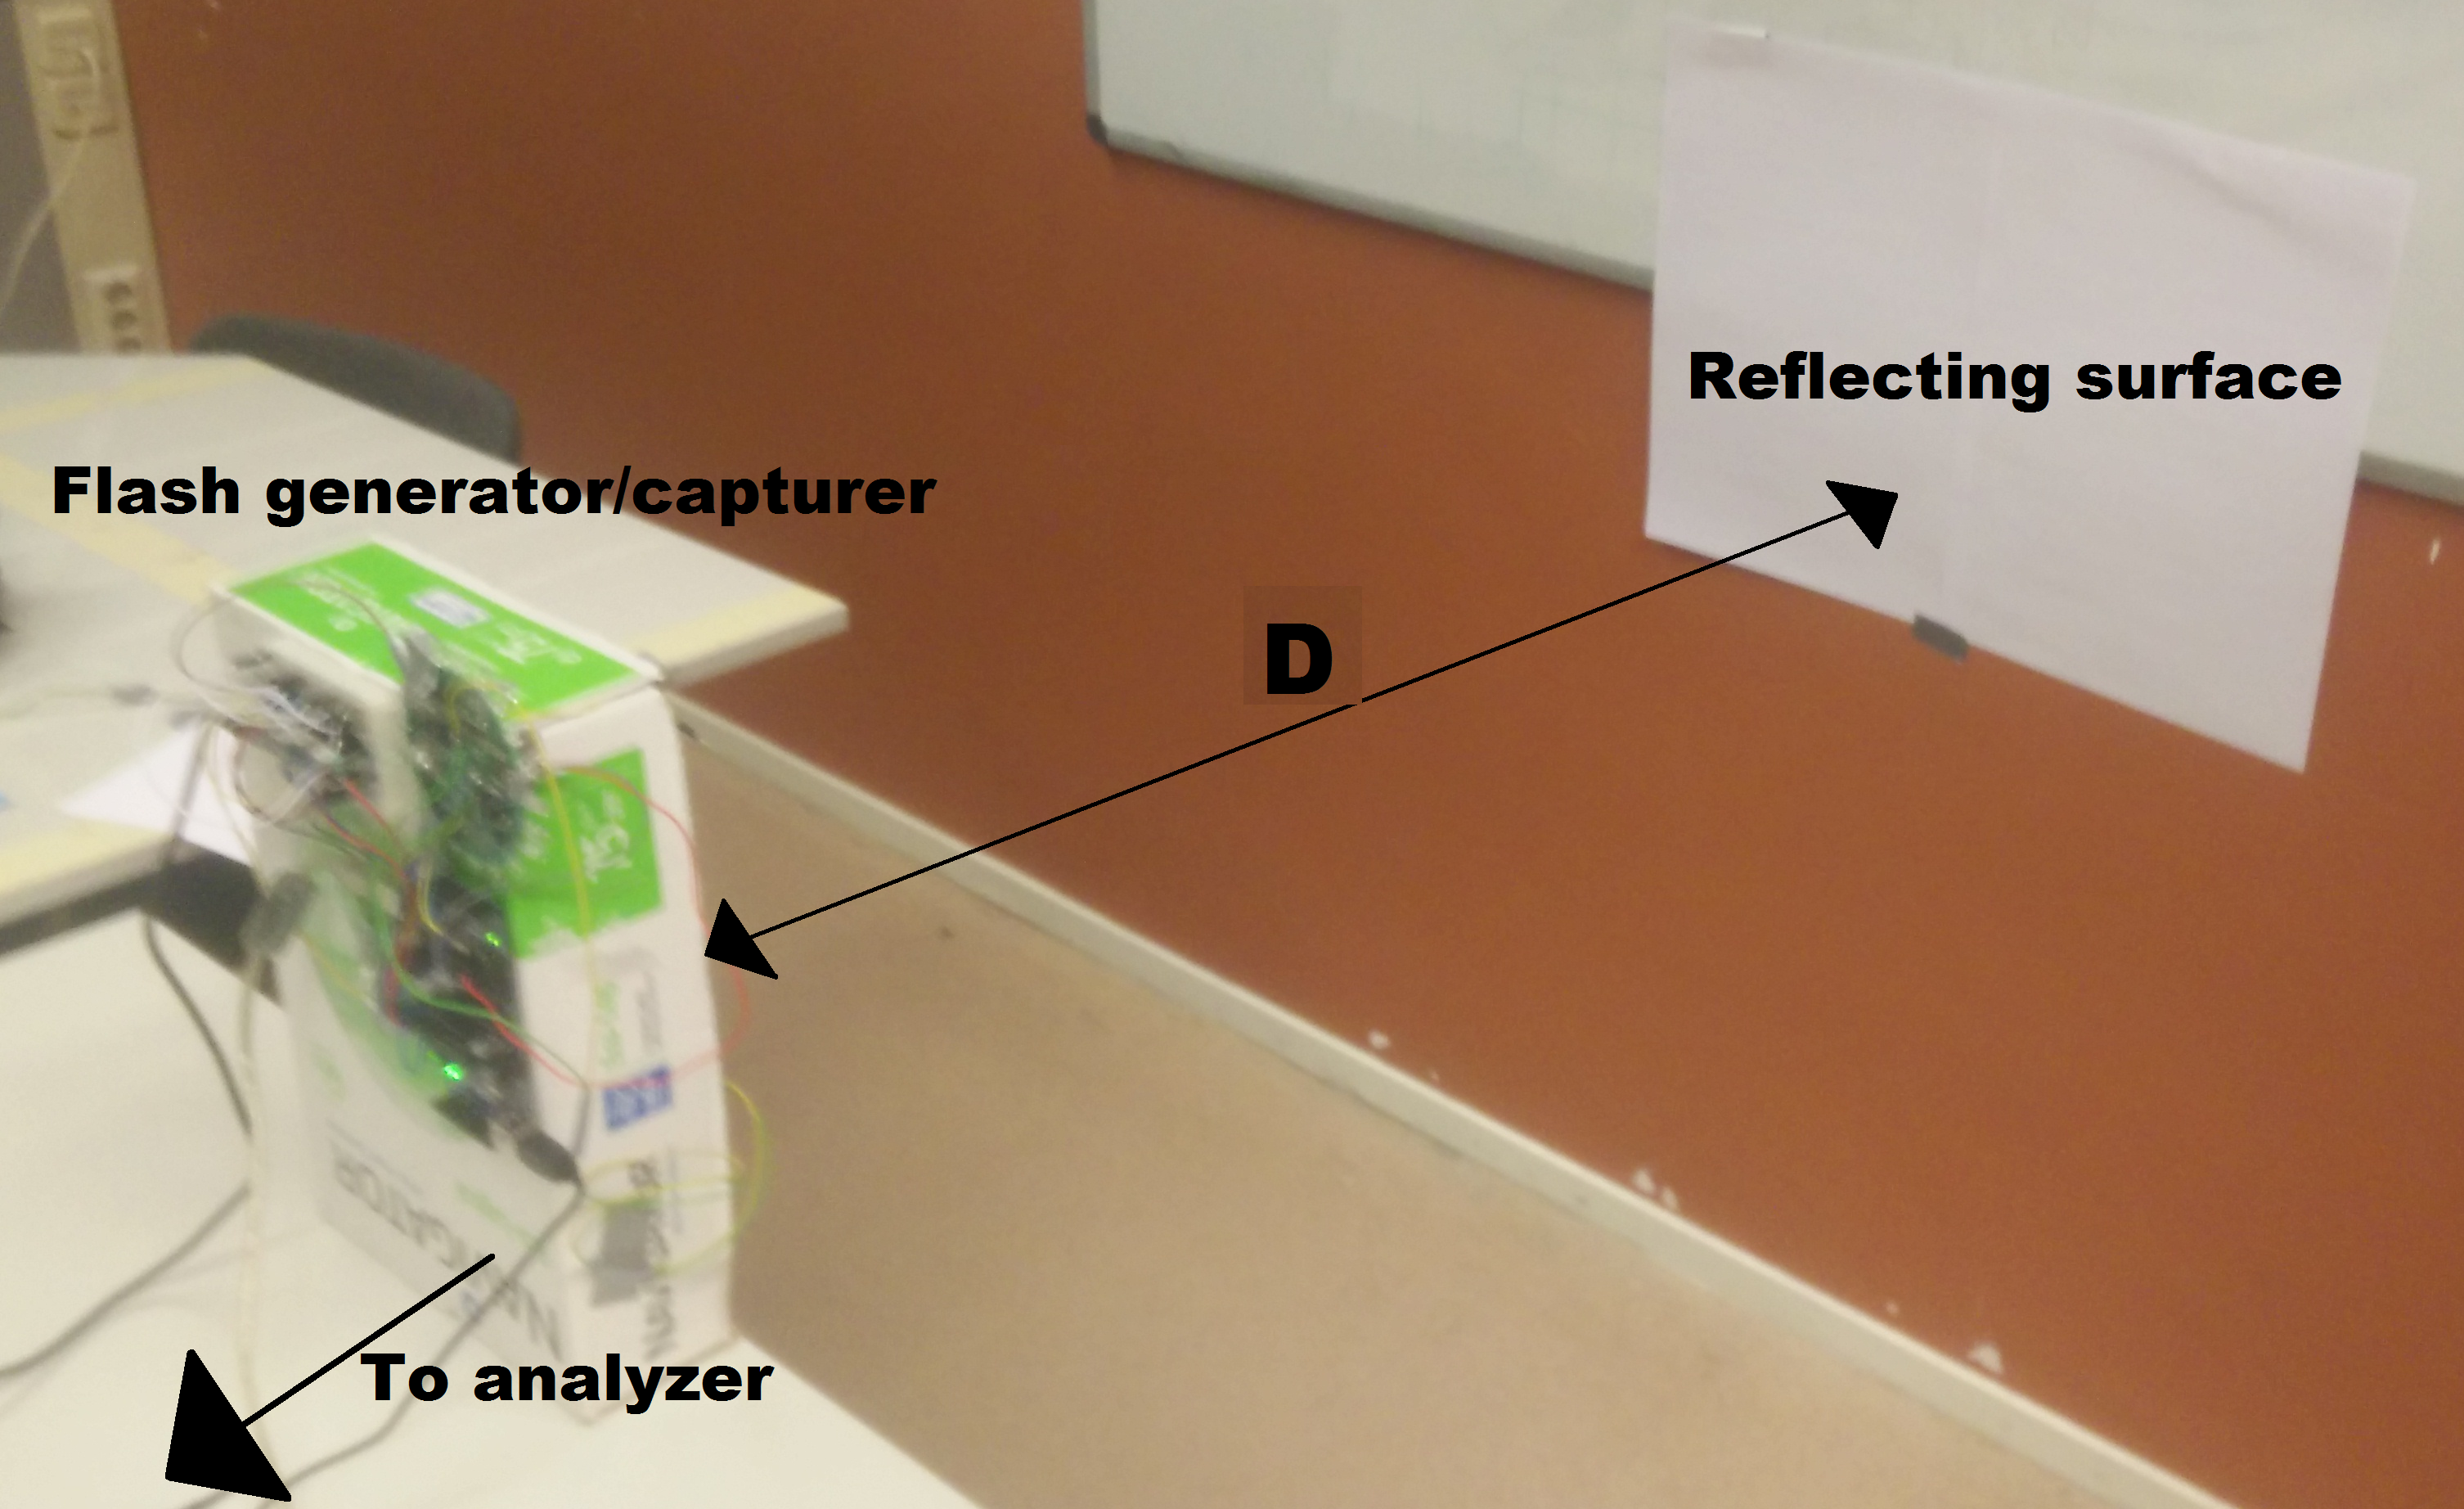
\includegraphics[width=60mm]{pics/Flashcapture_light.png}}
	\subfigure[Test set-up in dark environment]{\label{fig:Flashcapture_dark}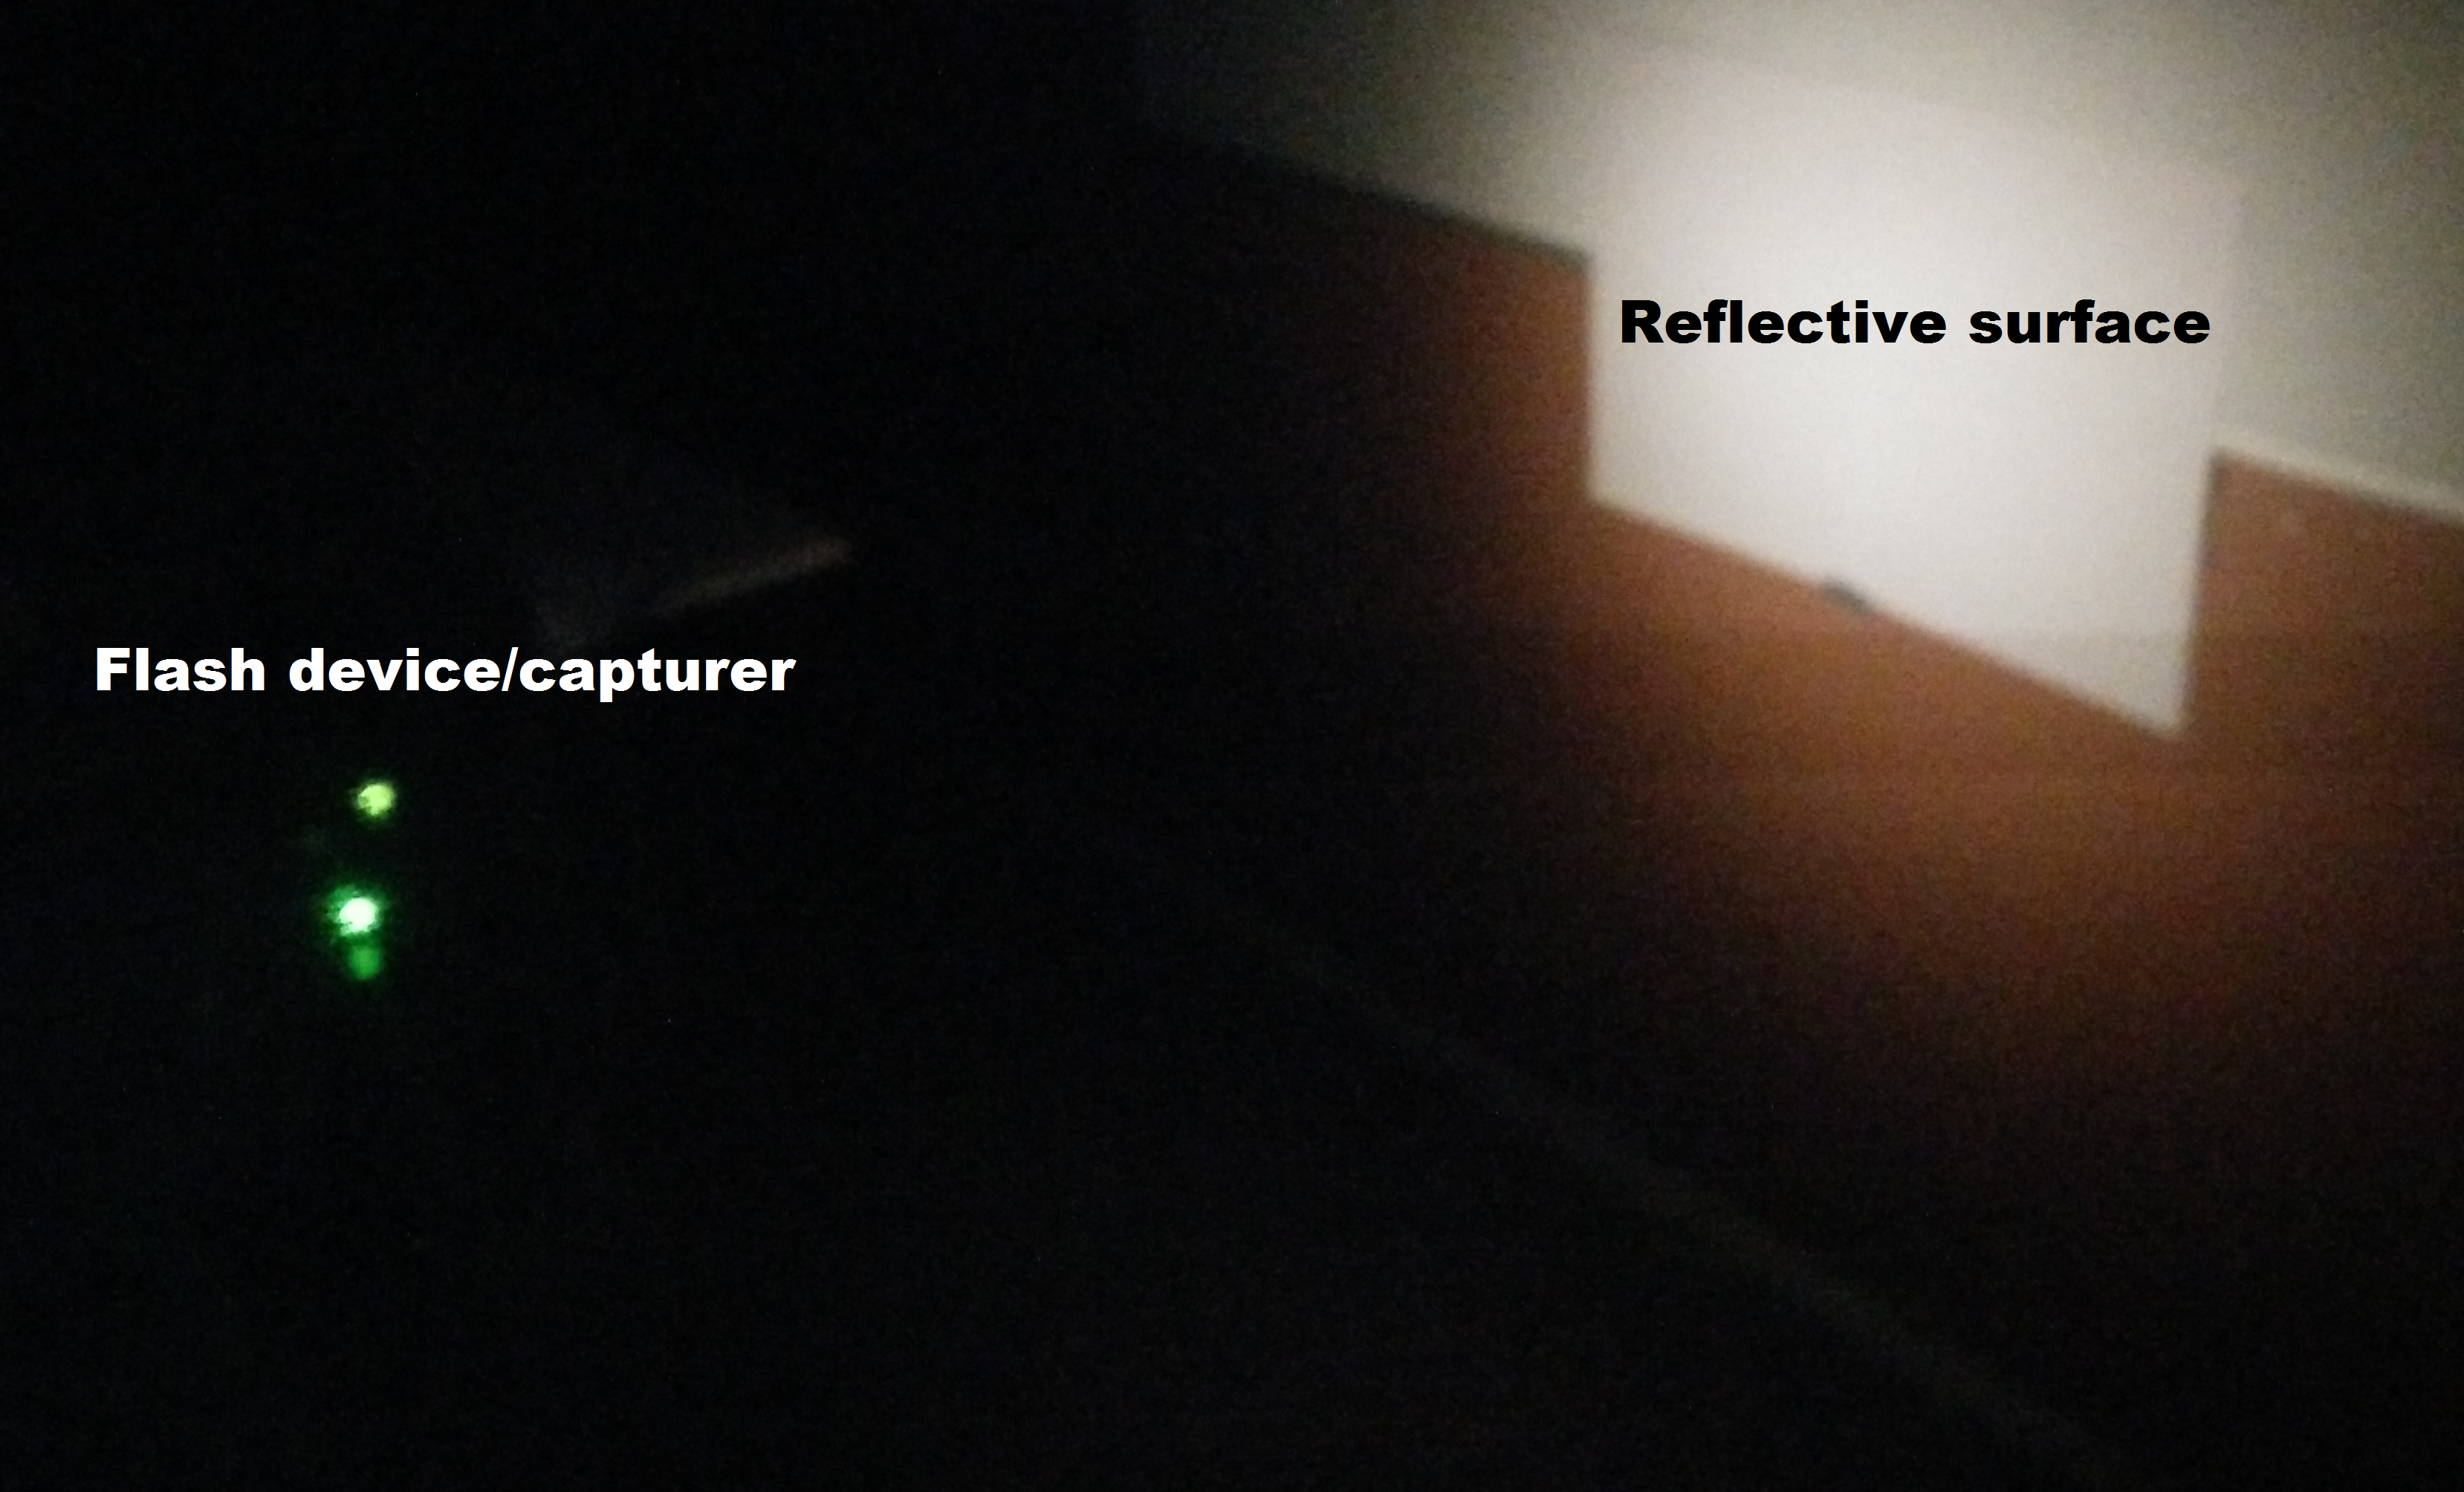
\includegraphics[width=60mm]{pics/Flashcapture_dark.png}}
	\caption{Test set-up used to capture flashes in the darkroom.\label{fig:Flashcapturing}}
\end{figure}

\section{Flash properties}
\label{sec:Flash_generator}
The test set-up has several parameters which can affect the perceived flash: $T_{on}$ (on time of the LED), $I$ (brightness of the LED), $S_{PD}$ (sensitivity of the photodiode) and $D$ (distance between device and reflecting surface). This section shows how each of these parameters influences the received signal. Note that the period, $T$, is not present in the list as should not influence an individual flash as long as the flashes are not too close together.

Figure \ref{fig:InfOfTon} shows several responses for different $T_{on}$. The Figure shows that all signals closely match each other, until the light is turned off. This is a useful property as this means it's possible to reduce the $T_{on}$ with no influence on the signal, if the ending of the flash is not used.

Figure \ref{fig:InfOfI} shows the influence of using the different amplification circuits of the flash generator. It can be seen that the LED powered with more current (because of the smaller resistor) is perceived as brighter to the system than the lights powered with a smaller current. It's also observed that the LED powered with higher currents show up earlier to the system. This is because LEDs driven with higher currents turn on faster \cite{LED_on}. This means that if a lower LED current is used a bigger $T_{on}$ is required to obtain useful information.

Figure \ref{fig:InfOfD} shows a set of measured flashes at a variety of distances from the wall. It clearly shows that if the distance increases, the observed light decreases. This is logical, as when light travels longer distances, the relative intensity of the light decreases. 

Figure \ref{fig:InfOfPD} shows what happens when the different photodiodes are used. As expected, the RSS rises once we increase the gain on the photodiode. $S_{PD_3}$ almost instantly saturates as the gain is too strong when used in combination with $I_1$. $S_{PD_3}$ is therefore also displayed with in combination with $I_3$. Another noticeable change is the frequency of the ripple, caused by the amplifier. This change is expected, as the resistor in the feedback loop of the amplifier was changed.

\begin{figure}
	\centering     %%% not \center
	\subfigure[]{\label{fig:InfOfTon}\includegraphics[width=60mm]{pics/InfluenceOfTon.png}}
	\subfigure[]{\label{fig:InfOfI}\includegraphics[width=60mm]{pics/InfluenceOfI.png}}
	\\
	\subfigure[]{\label{fig:InfOfD}\includegraphics[width=60mm]{pics/InfluenceOfD.png}}
	\subfigure[]{\label{fig:InfOfPD}\includegraphics[width=60mm]{pics/InfluenceOfPD.png}}
	\caption{Several perceived flashes generated with different settings of $T_{on}$, $I_{LED}$, $D$ and $S_{PD}$.\label{fig:InfOf}}
\end{figure}

% properites checklist:
% - What happens if distance increases
%   + fig with multiple distances
% - What happens if t-on time increases
%   + fig with increasing t-on
% - What happens if intensity increases
%   + fig multiple 3 intensities
% sumarize in table 
% conclude:
% - 

\section{Flash features}
This section explores what kind of features can be extracted from a flash signal. It will then compare the methods based on required $T_{on}$, precision, detectability and computational complexity.

\subsection{Feature considerations}
The maximum of a flash response could contain useful information. Even though the light at the first maximum has not fully turned on yet, it still is some measure of the perceived light. This can be especially useful if the maximum of the flash always occurs at the exact same moment in time relative to the light turning on. If that's the case, then the maximum value of the first peak could provide us with enough information of the environment. If the maximum value of the first peak holds enough information, then a very small $T_{on}$ can be used to obtain this value, as decreasing $T_{on}$ does not significantly influence the height and form of the first peak.

Another possibility is to remove the oscillation of the signal with a low pass filter and then take the maximum value of the filtered signal. This method is less reliant on precise timing of the pulse. It also uses more samples of the signal and should therefore be able to obtain a value which better represents the reflections of the current environment than the maximum method. A downside to this method is that a filter designed to deal with one frequency of ripple, is not immediately suited to deal with the ripple frequencies of the other amplifiers

Another method considered is to use the area underneath the flash. This method has the advantage of being both simple and flexible. It does not matter if $T_{on}$ is chosen big or small, it will always give a reliable result if $T_{on}$ is not changed. It also does not care about the ripple frequency of the amplifier. This method simply sums all information available to obtain a measure of the reflections.

The final possibility considered is the filtered sum method. It first uses a filter to smooth the signal to then calculate the surface underneath it. It also requires multiple filters to be designed (one for each $S_{PD}$ amplifier). It might however give a more detailed result than the filter method, as more information is used obtaining the data point.

\subsection{Feature comparison}
A test was created to compare the effectiveness of each feature with various settings in a full scale environment ($D = 280cm$). All of the features where extracted by the flash receiver simultaneously from consecutive flashes. The test was executed as follows:
\begin{enumerate}[itemsep=-1ex]
	\item Set the parameters for the given test ($S_{PD}$, $I$, $T_{on}$).
	\item Move a highly reflective piece of cloth underneath the set-up at $185cm$ ($D = 95cm$).
	\item Move the piece of cloth underneath the set-up again, but now from the other direction.
	\item Calculate the \textit{detectability} $Q$, of the received signal.
\end{enumerate}
If we refer to the \textit{'detectability'} in this thesis we mean $Q$ as defined in equation \ref{eq:snr}. This equation calculates ratio between the standard deviation of the signal when nothing is passing by and the absolute minimum and maximum of when something is. The higher $Q$, the easier the signal should be to distinguishable from noise.

\begin{equation}
Q(PD) = \left(\frac{\mu(PD_{NoEvent}) - min(PD_{event})}{\sigma(PD_{NoEvent})} + \frac{ max(PD_{event}) - \mu(PD_{NoEvent})}{\sigma(PD_{NoEvent})}\right)
\end{equation}
\begin{equation}
\label{eq:snr}
Q(PD) = \frac{max(PD_{Event}) - min(PD_{Event})}{\sigma(PD_{NoEvent})} 
\end{equation}

The test was done with all combinations of $S_{PD}$ and $I$. Only the combinations of $PD_2, I_{1}$ and $PD3, I_{3}$ gave potential usable results at full scale as for other combinations the flash was invisible or too bright (saturation) to observe. Several consecutive captured features can be seen in the Figures \ref{fig:SimpleFeatures} and \ref{fig:complexFeatures}. These where then used to calculated $Q$ for each scenario. An overview of all detectability values can be seen in table \ref{SNR_results}.

Based on the results of the $Q$ test it was chosen to use the Filtered sum method with $T_{on} = 200\mu s$. This method gives better results than the maximum and filtered maximum methods because more measurements are used to determine the final value, leading to lower standard error. The reason that this method works better than the sum method lies in the fact that the filtered signal is a better representation for the environment that the rippled signal. This can also be seen in the difference between the maximum and filtered maximum.

\begin{table}[]
	\centering
\begin{tabular}{l|lll|lll|}
	& \multicolumn{3}{c|}{$Q$: $S_{PD_2}, I_1$} & \multicolumn{3}{c|}{$Q$: $S_{PD_3}, I_3$} \\
	$T_{on}$         & $150 \mu s$ & $200\mu s$ & $250\mu s$ & $150\mu s$  & $20\mu s$  & $25\mu s$  \\ \hline
	Maximum          & 35          & 38         & 40         & 5           & 5          & 5          \\
	Filtered maximum & 39          & 65         & 66         & 20          & 27         & 33         \\
	Sum              & 45          & 75         & 95         & 18          & 20         & 26         \\
	Filtered sum     & 50          & 105        & 100        & 19          & 20         & 24        
\end{tabular}
	\caption{Overview of the test results.\label{SNR_results}}
\end{table}


\begin{figure}
	\centering     %%% not \center
	\subfigure[]{\label{fig:simple_PD2}\includegraphics[width=60mm]{pics/SNR_simple_PD2.png}}
	\subfigure[]{\label{fig:simple_PD3}\includegraphics[width=60mm]{pics/SNR_simple_PD3.png}}
	\caption{Data extracted using the maximum and filtered maximum methods with $T_{on} = 250\mu s$.\label{fig:SimpleFeatures}}
\end{figure}

\begin{figure}
	\centering     %%% not \center
	\subfigure[]{\label{fig:complex_PD2}\includegraphics[width=60mm]{pics/SNR_complex_PD2.png}}
	\subfigure[]{\label{fig:complex_PD3}\includegraphics[width=60mm]{pics/SNR_complex_PD3.png}}
	\caption{Data extracted using the sum and filtered sum method with $T_{on} = 200\mu s$.\label{fig:complexFeatures}}
\end{figure}

\section{Flash period}
The final parameter to decide is the period of the signal, $T$. This value has no influence on the detectability of the signal. It has however a clear influence on how much light is used by the system, as decreasing $T$ directly increases the amount of flashes which occur. We can't choose a too low value for $T$ as then users will observe flickering of the light. Another reason $T$ can't be chosen too low is that certain kind of noise still needs to be filtered out of the system. It is almost guaranteed that some 50Hz component will be seen in the signal, as long as it's connected to the net. 

For these reasons, $T$ was chosen to be 800$\mu s$ resulting in a flash frequency of 125Hz. This frequency is high enough to filter the expected 50Hz noise. Even though literature recommends at least 200Hz to prevent the visibility of flickering, none was observed by 10 different test subjects with this setting of $T$.

\section{Conclusion}
In this chapter, several methods of extracting useful data from a flashes where presented. 
The Flash analyser will run at a frequency of 125Hz, a $T_{on}$ of $200\mu s$ with maximum light intensity $I_1$ using the filtered sum method with $S_{PD_2}$ to extract information from the reflections. These settings provide the best found detectability with the given platform. The next step for the project is creating an algorithm to analyse set of consecutive flashes.
\include{chapters/Algorithm}
\chapter{System evaluation}
\label{System_evaluation}
In the previous chapter an algorithm was presented, which could be capable of classifying a set of consecutive samples into two groups: Activity detected or no activity detected. The algorithm is however dependent on several values which have not been determined yet as they might, or might not be dependent on the operating environment. This chapter will therefore focus on finding the ideal values for several test environments and compare them with each other.

This chapter will first present the measures used for evaluating the system. It will follow up with describing and evaluating several pedestrian test environments. It will then do the same for a scale model simulating a street and finalizes with summarising the results.

\section{Measures of evaluation}
The system will be evaluated on three different criteria: Precision, recall and and response time. Precision is defined in equation \ref{eq:precsion/recall} and gives us insight in how many situations the light would turn on unnecessarily. Recall is defined in equation \ref{eq:precsion/recall} and gives us insight in how often the light fails to turns on when an object passes by. 

\begin{equation}
\label{eq:precsion/recall}
Precision = \frac{TP}{TP + FP}
\quad
Recall = \frac{TP}{TP + FN}
\end{equation}
The precise repose time is impossible to determine with the used dataset, as the starting time of the event is not defined. It is however possible that if two different settings of algorithms trigger a detection, we compare the detection times with each other.

\section{Hallway Evaluation}
This section evaluates the system on detecting pedestrians walking by through a hallway. It will first explain the test set-up and procedure, followed by a section showing the ideally found algorithm settings and their detection results.

\subsection{Test set-up}

\begin{figure}
	\includegraphics[width=\textwidth]{pics/Evaluation_paths.png}
	\caption{The three paths the test subjects had to walk underneath the light.}
	\label{fig:Evaluation_paths}
\end{figure}

\begin{figure}
	\centering     %%% not \center
	\label{fig:TestPicture}
	\subfigure[Indoor]{\label{fig:setup_a}\includegraphics[width=60mm]{pics/Setup_outdoor.jpg}}
	\subfigure[Outdoor]{\label{fig:setup_b}\includegraphics[width=60mm]{pics/Setup_outdoor.jpg}}
	\caption{Pictures of the test set-up indoor (a) and outdoor (b). The light was suspended at 2.6m high.}
\end{figure}

\subsection{Results}

\begin{table}[]
	\centering
\begin{tabular}{l|llllllllllll}
	& d   & m   & l & L & T   & k   & $P_{set1}$ & $P_{set2}$ & $P_{set1,2}$ & $R_{set1}$ & $R_{set2}$ & $R_{set1,2}$ \\ \hline
	Heuristic                                                    &     &     &   &   &     &     &            &            &              &            &            &              \\ \hline
	\begin{tabular}[c]{@{}l@{}}Evolution \\ set 1\end{tabular}   & 539 & 654 & 4 & 4 & 3.5 & 0.1 &            &            &              &            &            &              \\ \hline
	\begin{tabular}[c]{@{}l@{}}Evolution\\ set 2\end{tabular}    &     &     &   &   &     &     &            &            &              &            &            &              \\ \hline
	\begin{tabular}[c]{@{}l@{}}Evolution\\ set 1, 2\end{tabular} & 475 & 714 & 4 & 4 & 4.5 & 0.8 &            &            &              &            &            &             
\end{tabular}
	\caption{Results of the hallway tests\label{tbl:hallwayresults}}
\end{table}

\section{Street}
This section evaluates the system on detecting cars driving by on a road with a scale model. It will first explain the test set-up and how it was scaled. It then explains the test procedure, followed by a section showing the ideally found algorithm settings and their detection results.

\subsection{Test set-up}
The street scenario is was tested with a scale model. The dimensions of the scale model where determined with equations X to Y. Equation \ref{PD_FS} represents an approximation of the strength of the received signal. It 


\begin{equation}
\label{PD_FS}
	PD_{fullscale} = \frac{E_{hor} * S_{car}}{H^2} = \frac{3 * 1}{7^2}
\end{equation}

\begin{equation}
\label{PD_S}
	PD_{scale} = \frac{I_L * \frac{1}{39}}{H^2}
\end{equation}

\subsection{Results}

\section{Conclusion}

% CONCLUSIONS AND FUTURE WORK
\chapter{Conclusions and Future Work}
\label{chp:conclusionsandfuturework}

\section{Conclusions}
TODO CONCLUSIONS
 - It works with crappy hardware
 - 

	

\section{Future Work}
The present work severs as a proof of concept for detecting activity in the line of sight of an LED. I personally think that the potential of this system is huge, especially if a dedicated platform is created. Below I have listed several ideas for future research, which I think have great potential, if a proper platform is created and it would be awesome if anyone would the dark sensing project to the next level.

\begin{itemize}
	\item \textbf{Multiple units in one room} - The algorithm is currently designed for a stand-alone device. If we would hang multiple of these systems in the same room then it's likely that some of the light flashes overlap and trigger a false positives regularly. This problem could be solved by having each detector flash in another timeslot, but this requires more research.
	\item \textbf{Tracking} - The system is currently only detecting activity. It could also be expanded for other purposes. It might for example be possible to use multiple photo diodes, lenses or field of view blockers to track bypassing pedestrians.
	\item \textbf{A dark sensing network} - Multiple working units in one room is nice, but multiple units working together to track, predict and illuminate the path of a pedestrian is nicer. This could be achieved by having the devices communicate using the flashes already generated by the device (visible light communication).
\end{itemize}

% BIBLIOGRAPHY
%#define SORTED 1
\bibliographystyle{bib/latex8}
\bibliography{bib/mycollection}

\appendix

\chapter{Code repository}
\label{app_repository}
This appendix is the github repository where all the raw data, code and MATLAB scripts can be found, used to create this thesis. It can be found at:  \url{https://github.com/hkleingeld/DarkSensing}.


\chapter{Raw Model results}
\label{app:RawModelResults}
This appendix contains the raw results of the model.

\begin{table}[]
	\hspace{-15mm}
	\label{tab:results_hallway}
	\begin{tabular}{llllllllll}
		y   & H                         & \begin{tabular}[c]{@{}l@{}}min\\ $\alpha = 0.2$\end{tabular} & \begin{tabular}[c]{@{}l@{}}max\\ $\alpha = 0.2$\end{tabular} & \begin{tabular}[c]{@{}l@{}}min\\ $\alpha = 0.3$\end{tabular} & \begin{tabular}[c]{@{}l@{}}max\\ $\alpha = 0.3$\end{tabular} & \begin{tabular}[c]{@{}l@{}}min\\ $\alpha = 0.4$\end{tabular} & \begin{tabular}[c]{@{}l@{}}max\\ $\alpha = 0.4$\end{tabular} & \begin{tabular}[c]{@{}l@{}}min\\ $\alpha = 0.5$\end{tabular} & \begin{tabular}[c]{@{}l@{}}max\\ $\alpha = 0.5$\end{tabular} \\ \cline{3-10} 
		0m   & \multicolumn{1}{l|}{1.4m} & -0.08 & 0.70  & -0.03 & 1.30  & 0     & 1.90  & 0     & 2.50  \\
		& \multicolumn{1}{l|}{1.6m} & -0.07 & 1.60  & -0.02 & 2.66  & 0     & 3.73  & 0     & 4.80  \\
		& \multicolumn{1}{l|}{1.8m} & -0.06 & 3.46  & -0.01 & 5.54  & 0     & 7.61  & 0     & 9.69  \\
		0.2m & \multicolumn{1}{l|}{1.4m} & -0.05 & 0.65  & -0.01 & 1.17  & 0     & 1.70  & 0     & 2.23  \\
		& \multicolumn{1}{l|}{1.6m} & -0.05 & 1.34  & 0     & 2.22  & 0     & 3.11  & 0     & 3.99  \\
		& \multicolumn{1}{l|}{1.8m} & -0.04 & 2.64  & 0     & 4.24  & 0     & 5.83  & 0     & 7.43  \\
		0.4m & \multicolumn{1}{l|}{1.4m} & -0.07 & 0.28  & -0.02 & 0.59  & 0     & 0.90  & 0     & 1.21  \\
		& \multicolumn{1}{l|}{1.6m} & -0.07 & 0.56  & -0.02 & 1.01  & 0     & 1.46  & 0     & 1.91  \\
		& \multicolumn{1}{l|}{1.8m} & -0.07 & 0.91  & -0.02 & 1.59  & 0     & 2.26  & 0     & 2.93  \\
		0.6m & \multicolumn{1}{l|}{1.4m} & -0.08 & 0.04  & -0.03 & 0.18  & -0.01 & 0.33  & 0     & 0.47  \\
		& \multicolumn{1}{l|}{1.6m} & -0.09 & 0.09  & -0.04 & 0.27  & -0.01 & 0.44  & 0     & 0.62  \\
		& \multicolumn{1}{l|}{1.8m} & -0.10 & 0.05  & -0.05 & 0.26  & -0.01 & 0.47  & 0     & 0.68 
	\end{tabular}
	\caption{Differences with baseline (no object) for each simulated situation}
\end{table}

\begin{table}[]
	\centering
	\label{tab:results_street_car}
	\begin{tabular}{llllll}
		y & Colour & \begin{tabular}[c]{@{}l@{}}min\\ $\alpha = 0.06$\end{tabular} & \begin{tabular}[c]{@{}l@{}}max\\ $\alpha = 0.06$\end{tabular} & \begin{tabular}[c]{@{}l@{}}min\\ $\alpha = 0.14$\end{tabular} & \begin{tabular}[c]{@{}l@{}}max\\ $\alpha = 0.14$\end{tabular} \\ \cline{3-6} 
			1.5m & \multicolumn{1}{l|}{Silver} &  &  &  &  \\
			& \multicolumn{1}{l|}{Black} &  &  &  &  \\
			& \multicolumn{1}{l|}{Red} &  &  &  &  \\
			4.5m & \multicolumn{1}{l|}{Silver} &  &  &  &  \\
			& \multicolumn{1}{l|}{Black} &  &  &  &  \\
			& \multicolumn{1}{l|}{Red} &  &  &  & 
	\end{tabular}
	\caption{Differences with baseline (no object) for each simulated situation}
\end{table}

\begin{table}[]
	\centering
	\label{tab:results_street_human}
	\begin{tabular}{llllll}
		\begin{tabular}[c]{@{}l@{}}Object\\ albedo\end{tabular} & H & \begin{tabular}[c]{@{}l@{}}min\\ $\alpha = 0.06$\end{tabular} & \begin{tabular}[c]{@{}l@{}}max\\ $\alpha = 0.06$\end{tabular} & \begin{tabular}[c]{@{}l@{}}min\\ $\alpha = 0.14$\end{tabular} & \begin{tabular}[c]{@{}l@{}}max\\ $\alpha = 0.14$\end{tabular} \\ \cline{3-6} 
		0.1 & \multicolumn{1}{l|}{1.8m} &  &  &  &  \\
		& \multicolumn{1}{l|}{1.6m} &  &  &  &  \\
		& \multicolumn{1}{l|}{1.4m} &  &  &  &  \\
		0.4 & \multicolumn{1}{l|}{1.8m} &  &  &  &  \\
		& \multicolumn{1}{l|}{1.6m} &  &  &  &  \\
		& \multicolumn{1}{l|}{1.4m} &  &  &  & 
	\end{tabular}
	\caption{Differences with baseline (no object) for each simulated situation}
\end{table}
\chapter{Flash analyser schematics}
\label{app_schematics}
This appendix contains pictures of electronic schematic created for specifically the flash analyser. Schematics of the processor boards where not added, as only small changes small modifications (see section \ref{chp:Platform}) where made to these boards. The original scematics can be found at:
\begin{itemize}
    \item Flash analyser - \url{https://github.com/LennartKlaver/SDVN1} 
    \item LED controller - \url{https://www.arduino.cc/en/uploads/Main/arduino-uno-schematic.pdf}
\end{itemize}


\section{LED driver}
\begin{figure}[!h]
	\includegraphics[width=\textwidth]{pics/LED_Driver.png}
	\caption{Drivers used to drive the LED.}
	\label{fig:LED_Driver}
\end{figure}

\section{Interfaces between components}
@TODO!

\end{document}

